\documentclass[oneside, class=book, 12pt, crop=false]{standalone}

\usepackage{../dissertationstyle}

\bibliography{../personal}

\begin{document}

\resetfigpath{preparation}

\ifstandalone
  \graphicspath{ {./images/} }
  \setcounter{chapter}{1}
  \chapter{Preparation}
\fi


%Structure:
%
%Explain 
%
%Talk about data collection (which pieces were used)
%
%Talk about preparatory work done for understanding DSP techniques, as well as Ellis' beat-tracking system.
%
%Choice of metrics: mention not using symbolic data makes it more difficult to get metrics that work has previously been done on
%
%Requirements analysis:
%
%
%remember:
%
%reverb, echo, non-linear frequency response, fix by multiplying by inverse?


%%%%%%%%%%%%%%%%%%%%%%

This chapter gives and discusses the preparatory work done for this project. We begin by explaining some key concepts and algorithms used in this project. Next, we discuss and justify choices made for real-world data collection and metric calculation. We then discuss the requirements of this project, and finally talk about the software engineering tools and techniques that were employed throughout this project.

\section{Digital Signal Processing Techniques}\label{section:dsp techniques}

First, we introduce some important DSP concepts and techniques: the Fourier transform, the discrete time Fourier transform, the discrete Fourier transform, and the mel scale.

In DSP, we can model an analog signal as a continuous function of time $x(t)$, and a digital signal as a discrete sequence $\{x_n\} = \ldots, x_{-2}, x_{-1}, x_0, x_1, x_2, \ldots$, essentially a list of numbers. With a sampling period $t_s$ we can sample an analog signal $x(t)$ to generate a digital signal $\{x_n\}$ as follows: $\{x_n\} = x(nt_s)$, or equivalently with sampling period $f_s$ we get $\{x_n\} = x(\frac{n}{f_s})$

\subsection{The Fourier Transform}\label{section:fourier transform}

An important operation in DSP is the Fourier transform, which allows us to convert a signal from the time-domain into the frequency-domain. The Fourier transform $X(f) = \mathcal{F}\{x(t)\}$ is defined  on a continuous signal $x(t)$ in Equation \ref{eq:ft}

\begin{equation}\label{eq:ft}
  X(f) = \mathcal{F}\{x(t)\}(f) = \int_{-\infty}^\infty x(t)e^{-j2\pi ft}\mathrm{d}t
\end{equation}

Here, the symbol $j$ refers to $\sqrt{-1}$. By rewriting $e^{-j2\pi ft}$ as $\cos(2\pi f t) - j\sin(2\pi f t)$ we get the definition in Equation \ref{eq:ft2}, which should make the purpose of this transform clearer:

\begin{equation}\label{eq:ft2}
  X(f) = \mathcal{F}\{x(t)\}(f) = \int_{-\infty}^\infty x(t)[\cos(2\pi ft) - j\sin(2\pi f t)] \mathrm{d}t
\end{equation}

Here, it is more obvious that we are taking the frequency content of $x(t)$. It should be noted that the Fourier transform generates complex values. However, if the signal $x(t)$ is both real and even, then its Fourier transform $X(f)$ will also be real and even. Subsequently, if $X(f)$ is real and even, then the values for negative $f$ contain the same information as the values for non-negative $f$, so we can purely consider real, non-negative frequencies, which makes interpreting the Fourier transform in a real-world sense easier.

As an example, we provide the Fourier transform of the box function in Figure \ref{fig:ft example}.

\begin{minipage}{\textwidth}
\begin{minipage}{.5\textwidth}
    \begin{tikzpicture}[
      declare function={
          func(\x)= (\x<=-1) * (0)   +
         and(\x>-1, \x<=1) * (1)     +
         (\x>1) * (0);
      }
    ]
    \begin{axis}[
      axis x line=middle, axis y line=middle,
      ymin=-1, ymax=2, ytick={-1,...,2}, ylabel=$x(t)$,
      xmin=-2, xmax=2, xtick={-2,...,2}, xlabel=$t$,
    ]
    % lol
    \addplot[blue, domain=-2:2, samples=100]{func(x)};
    \end{axis}
    \end{tikzpicture} 
\end{minipage}%
\begin{minipage}{.5\textwidth}
    \begin{tikzpicture}[
      declare function={
          func(\x) = sin(deg(\x))/(\x);
      }
    ]
    \begin{axis}[
      axis x line=middle, axis y line=middle,
      ymin=-1, ymax=2, ylabel=$X(f)$,
      xmin=-10, xmax=10, xlabel=$f$,
    ]
    % lol
    \addplot[blue, domain=-10:10, samples=100]{func(x)};
    \end{axis}
    \end{tikzpicture} 
\end{minipage}
\captionof{figure}{The rectangular function and its Fourier transform}\label{fig:ft example}
\centering
\end{minipage}


\subsection{The Discrete Time Fourier Transform and Discrete Fourier Transform}

For our work, we do not use continuous signals, we instead work with discrete sequences, and as such we need a variant of the Fourier transform to work with these discrete sequences. This is called the discrete time Fourier transform (DTFT), and the definition given in Equation \ref{eq:dtft} comes from considering our discrete sequence $\{x_n\}$ as being sampled from some continuous signal at sampling frequency $f_s$:

\begin{equation}\label{eq:dtft}
  \hat{X}(f) = \mathcal{F}\{\{x_n\}\}(f) = \sum_{-\infty}^\infty x_n \cdot e^{-2\pi j \frac{f}{f_s}n}
\end{equation}

In practice, we make one further restriction on our input sequences: they are finite. Fortunately, a useful property of the Fourier transform (that also holds for the DTFT) is that if the input is periodic, then the resulting spectrum will be discrete. So, we can take our finite input sequence, and turn it into an infinite, periodic, discrete sequence, and then take the DTFT to get a discrete frequency spectrum, which gives us the discrete Fourier transform (DFT).

This does not require much work to calculate, and for a finite sequence $x_0, \ldots, x_{N-1}$, we simply replace the bounds on our sum in Equation \ref{eq:dtft} with 0 and $N-1$, to get the definition of the DFT in Equation \ref{eq:dft}:

\begin{equation}\label{eq:dft}
  X_k = \sum_{n=0}^{N-1} x_n e^{-2\pi j \frac{k}{N}n}
\end{equation}


\subsection{The Mel Scale}

The mel scale is a scale of frequencies that intends to map distance between frequencies to differenecs in perceptual pitch. This is useful for this project, since the quantity we actually care about is pitch, and not Hertz frequency.

There are many different definitions for the mel scale, since perceptual pitch is a relatively subjective meausre, but we use the definition in Equation \ref{eq:mel}, where $f$ is a frequency in Hertz and $m$ is the corresponding frequency in the mel scale:

\begin{equation}\label{eq:mel}
  m = 2595\log_{10}\left(1 + \frac{f}{700}\right)
\end{equation}

\subsection{Convolution}

Convolution is a method of combining two signals that in essence combines the shape of both functions. It works by reversing one of the signals and sliding it over the other, computing the dot product for each shift.

We give the formula for convolution of two discrete sequences $\{x_n\} * \{y_n\} = \{z_n\}$ in Equation \ref{eq:convolution}, although there is a continuous analogue. Figure \ref{fig:convolution} gives a graphical representation of convolution.

\begin{equation}\label{eq:convolution}
    z_n = \sum_{k=-\infty}^\infty x_k \cdot y_{n-k}
\end{equation}

\begin{minipage}{\linewidth}
    \centering
\begin{minipage}{0.33\linewidth}
    \centering
  \begin{tikzpicture}[scale=0.5]
  \begin{axis}[
    ymin=0,
    xmin=0,
    xmax=7,
    xticklabels={,,},
    yticklabels={,,},
    ytick distance={0.125},
    ]
    \addplot[only marks] coordinates {
        (0, 0)
        (1, 1)
        (2, 0.5)
        (3, 0.25)
        (4, 0)
        (5,0)
        (6,0)
        (7,0)
      };

    \addplot +[mark=none, black, dashed] coordinates {(1, 1) (1,0)};
    \addplot +[mark=none, black, dashed] coordinates {(2, 0.5) (2,0)};
    \addplot +[mark=none, black, dashed] coordinates {(3, 0.25) (3,0)};

    \node[] at (axis cs: 5, 0.75) {\LARGE $\{x_n\}$};



      
  \end{axis}
    
\end{tikzpicture}
    
\end{minipage}%
\begin{minipage}{0.33\linewidth}
    \centering
  \begin{tikzpicture}[scale=0.5]
  \begin{axis}[
    ymin=0,
    xmin=0,
    xmax=7,
    xticklabels={,,},
    yticklabels={,,},
    ytick distance={0.125},
    ]
    \node[] at (axis cs: 5, 0.75) {\LARGE $\{y_n\}$};
    \addplot[only marks] coordinates {
        (0, 0)
        (1, 1)
        (2,0)
        (3,0)
        (4, 0.5)
        (5,0)
        (6,0)
        (7,0)
      };

    \addplot +[mark=none, black, dashed] coordinates {(1, 1) (1,0)};
    \addplot +[mark=none, black, dashed] coordinates {(4, 0.5) (4,0)};
  \end{axis}
    
\end{tikzpicture}
    
\end{minipage}%
\begin{minipage}{0.33\linewidth}
  \centering
  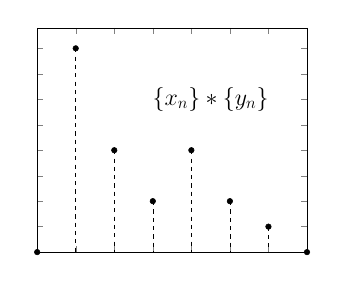
\begin{tikzpicture}[scale=0.5]
  \begin{axis}[
    ymin=0,
    xmin=0,
    xmax=7,
    xticklabels={,,},
    yticklabels={,,},
    ytick distance={0.125},
    ]
    \node[] at (axis cs: 4.5, 0.75) {\LARGE $\{x_n\} * \{y_n\}$};
    \addplot[only marks] coordinates {
        (0, 0)
        (1, 1)
        (2, 0.5)
        (3, 0.25)
        (4, 0.5)
        (5, 0.25)
        (6, 0.125)
        (7,0)

      };

    \addplot +[mark=none, black, dashed] coordinates {(1, 1) (1,0)};
    \addplot +[mark=none, black, dashed] coordinates {(2, 0.5) (2,0)};
    \addplot +[mark=none, black, dashed] coordinates {(3, 0.25) (3,0)};
    \addplot +[mark=none, black, dashed] coordinates {(4, 0.5) (4,0)};
    \addplot +[mark=none, black, dashed] coordinates {(5, 0.25) (5,0)};
    \addplot +[mark=none, black, dashed] coordinates {(6, 0.125) (6,0)};



      
  \end{axis}
    
\end{tikzpicture}
\end{minipage}
\captionof{figure}{Convolution of two discret sequences}
\label{fig:convolution}
\end{minipage}


\section{Beat Tracking}

Beat tracking is the technique of taking some audio signal of music, and attempting to find the location of beats, or the pulse, of the music. This is not the same as rhythm, since rhythm is more concerned with the location of individual notes, whereas beats are a steady pulse perceived by humans throughout a whole piece of music. The technique we use for beat tracking comes from a paper by Ellis \cite{ellis07} and makes use of dynamic programming techniques.

In this section, we give a brief overview of the algorithm. For an in-depth explanation, see Ellis' original paper \cite{ellis07}.

To perform beat tracking, we assume the existence of some onset function and a global tempo estimate, Ellis' constructions of which we explore further in Sections \ref{subsec:onset detection} and \ref{subsec:tempo inference} respectively. An onset function tracks where perceptual note onsets are in an audio signal as seen in Figure \ref{fig:onsetfunction}, and a tempo estimate is simply an estimate of how fast the piece is being played overall, in beats per minute (BPM).


The dynamic programming algorithm for beat tracking works by assuming we have some already optimal set of previous beat times, and then searching for the next beat time by trying to find a time with a high onset function value, as well as being coherent with the tempo estimate.



\begin{minipage}{\textwidth}
  \centering
  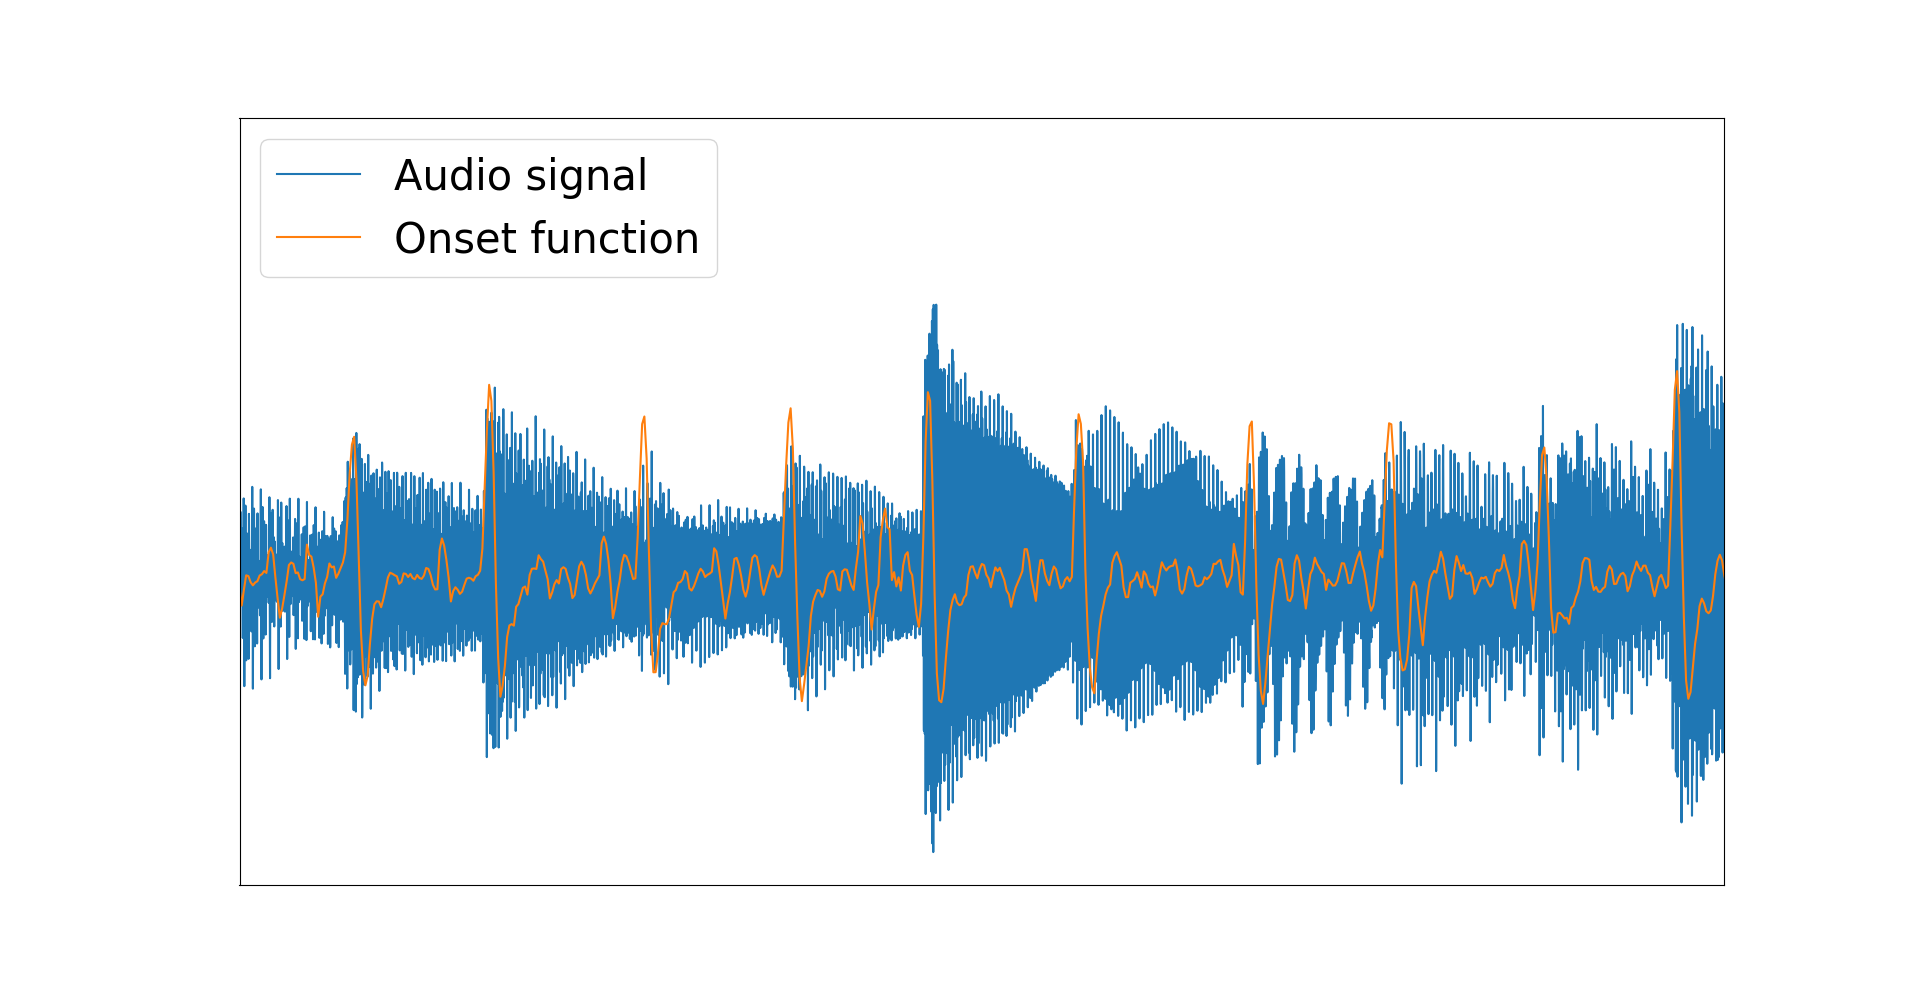
\includegraphics[scale=0.3]{onsetfunction}
  \captionof{figure}{Example onset function against audio signal}\label{fig:onsetfunction}
\end{minipage}

\subsection{Onset Detection}\label{subsec:onset detection}

 There is a wide literature on onset detection \cite{bello05}, but due to the nature of the relevant audio recordings (solo piano performances) which are relatively simple and have strong percussive elements, opting for the simple technique used by Ellis seemed sensible.

 The idea behind Ellis' onset function is to report a high value when there are large jumps in energy in multiple frequency bands, which indicates a note has been played.

 The general gist of the algorithm is as follows:

 \begin{itemize}

   \item
     Take windows of the sound, we use a 32ms wide window and advance by 4ms and compute their DFT in mel.

   \item
     Across all windows, compute the first-order difference for each pitch band, setting negative values to zero (so they do not interfere with the next step)

   \item
     For each pair of windows, sum all of the first-order differences together, such that we get a signal.

   \item
       Smooth and normalise the signal

 \end{itemize}

 The output of this is our onset function $O(t)$.


 \subsection{Tempo Inference}\label{subsec:tempo inference}

 The tempo inference algorithm is relatively simple, and uses our onset function.

 The idea is to iterate over a range of possible tempos, and for each tempo we compute $\tau$, the time between beats at that tempo. Then, we delay our onset function by $\tau$ to get $O(t - \tau)$, and compute the inner product between $O(t)$ and $O(t-\tau)$ to get a measure of how good our tempo guess was, since a good guess will hopefully align the peaks and thus result in a large inner product.

 We weight each of these inner products such that tempos closer to 120 BPM are get higher values (humans tend to gravitate towards this tempo), and then take the tempo with the highest value.




\section{Data Collection}


To evaluate the project, first-hand data had to be collected. The system requires multiple performances of the same piece by the same pianist, and generally performers tend to only ever upload one performance of a piece. This meant that I had to find both performers and pieces for them to perform, so that I could record them. Overall, there were 5 performers, each performing 4 pieces twice.

The subjects used all had experience in playing the piano, or else it would be unlikely that any unique nuances in playing could be found and identified. They were all experienced enough to be able to take a short excerpt of a piece of music, and be able to perform it well within a short time (around 15 minutes).

The pieces were chosen to be not too difficult, such that performers could learn them quickly, as well as be complex enough such that a reasonable amount of expressivity could be given in the performances. Furthermore, only short excerpts of the pieces were taken (around 8-16 bars). Scores of each of the excerpts are given in the appendix (TODO). The pieces chosen are given below:

\begin{itemize}
  \item Handel - Largo (from Xerxes)
  \item C418 - Sweden (transcribed by Torby Brand)
  \item Bach - Prelude in C Major
  \item Beethoven - Moonlight Sonata (1st Movement)
\end{itemize}

This selection of pieces also intends to cover a range of different techniques, e.g. `Prelude in C Major' has many fast notes in succession, whereas `Sweden' has slow chords.

Recordings were made by using a Kawai ES110 digital piano, recording directly into a computer, such that no noise or distortion from a microphone is present in the recordings.

\section{Metric Choice}

There are 5 metrics we use in this project, recall from Chapter \ref{chapter:introduction}:

\begin{itemize}
    \item
        Tempo variation over time

    \item
        Dynamics over time

    \item
        Chroma vector extraction

    \item
        Note offsets

    \item
        Timbre extraction
\end{itemize}

The data we have available to us is what informs these particular metric choices. A key factor is that we are dealing with raw audio signals, and not a symbolic representation like seen in previous work \cite{bernays14}. This means that certain luxuries are not afforded to us, like the ability to precisely see where note-ons and note-offs are, or the exact notes that are played, or where the sustain pedal is used. These choices were also informed by my own experience of playing and listening to solo piano music (note to John: is this point a good enough justification? Or do I need to find research that supports these metric choices more).

For example, with raw audio recordings we can make guesses at where notes are played (tempo variation over time, note offsets), and what notes are being played (chroma vector extraction), but we cannot know with certainty.

Furthermore, due to the system intended to work on performances of the same piece, we can try and measure qualities of a particular performer's interpretation of the piece with metrics like tempo variation over time and dynamics over time.

The timbre extraction metric, as explained before, is hard to give a semantic meaning for. It in essence works by taking the DFT of windows of the signal, and transformingeach of these DFTs with a discrete cosine transform (similar to the DFT) to obtain some coefficients for each window, yielding some form of spectrogram for the entire signal. 





\section{Requirements Analysis}

Table \ref{table:requirements} lists requirements and their priorities. These mirror the success criteria of the project.

\begin{minipage}{\textwidth}
  \centering
  \begin{tabular}{l|l}
    \textbf{Requirement} & \textbf{Priority}\\
    \hline
    \hline
    Calculators for each of the 5 proposed metrics & Necessary \\
    \hline
    Similarity scorers for each of the 5 proposed metrics & Necessary \\
    \hline
    Addition of optional variation to input data & Necessary \\
    \hline
    Code to automatically perform evaluation based on a plan & Preferable \\
    \hline
    Data synthesis engine to generate test piano data & Preferable \\
    \hline
    Data synthesis engine to generate test data from other instruments& Extension \\
    \hline
    Gathering of real-world piano performances & Necessary
  \end{tabular}
  \captionof{table}{}
  \label{table:requirements}
\end{minipage}


\section{Software Engineering Tools and Technologies}

\subsection{Programming Language and Libraries}

The system was developed entirely in Python3, and whilst having prior programming experience in Python was a benefit, the main draw to this language was the libraries available.

Python has available a number of libraries that allowed for fast development of the system, whilst being able to ignore implementation of algorithms/techniques that are not relevant to the project. In particular, the following modules were used:

\begin{itemize}
  \item
    \texttt{NumPy} and \texttt{SciPy}: the combination of both of these modules provide utility in that they provide frameworks for computing on large arrays of data, and implement algorithms for techniques like the DFT that allowed me to spend my time implementing core parts of the project.

  \item
    \texttt{Matplotlib}: This library allows for easy visualisation of large data sets, which resulted in both ease of debugging and presentation of data for evaluation.

  \item
    \texttt{fluidsynth}: This library allows for generating of audio files from a soundfont and symbolic data, which was useful for generating test audio data from scores.
    
\end{itemize}

\subsection{Version Control}

For version control, \texttt{git} was used and the repository was maintained on GitHub. Furthermore, a backup of the repository was periodically made and stored on a USB drive in case of failure.










\ifstandalone
  \printbibliography
\fi
    
\end{document}
